\documentclass[11pt]{article}

\usepackage{fullpage}
\usepackage{caption}
\usepackage{float}

\usepackage[T1]{fontenc}
\usepackage{textcomp}

\usepackage[english]{babel}
\usepackage[utf8]{inputenc}

\usepackage{lmodern}

\usepackage{hyperref}
\hypersetup{breaklinks}
\hypersetup{pdfborder=0 0 0}

\usepackage[babel=true]{microtype}


\usepackage{amsmath}
\renewcommand{\vec}[1]{\mathbf{#1}}
\newcommand{\mat}[1]{\mathbf{#1}}
\DeclareMathOperator{\Prob}{Prob}
\newcommand{\md}{\mathrm{d}}
\newcommand{\me}{\mathrm{e}}
\newcommand{\mT}{\mathrm{T}}

\usepackage{units}
\usepackage{tikz}
\usepackage[square,sort,comma,numbers]{natbib}
\usepackage{hypernat}

\allowdisplaybreaks[1]

\title{Supporting Information: \\
\textbf{Interactions between chronic diseases: asymmetric outcomes of co-infection at individual and population scales}}
\date{}
\author{Erin E. Gorsich$^{a,b*}$, Rampal S. Etienne$^{c}$, Jan Medlock$^{a}$, \\ Brianna R. Beechler$^{a}$, Johannie M. Spaan$^{b}$, Robert S. Spaan$^{d}$, \\Vanessa O. Ezenwa$^{e}$, Anna E. Jolles$^{a,b}$}

\begin{document}

\maketitle

\noindent{}a. Department of Biomedical Sciences, 105 Dryden Hall, Oregon State University \\
\noindent{}b. Department of Integrative Biology, Cordley Hall, Oregon State University \\
\noindent{}c. Groningen Institute for Evolutionary Life Sciences, University of Groningen, The Netherlands\\
\noindent{}d. Department of Fisheries and Wildlife, 104 Nash Hall, Oregon State University \\
\noindent{}e. Odum School of Ecology and Department of Infectious Diseases, College of Veterinary Medicine, University of Georgia \\
\noindent{}$\ast$ Corresponding author e-mail: eringorsich@gmail.com \\



\noindent \Large \textbf{Appendix 2. Additional information on model development and analysis}\\
\normalsize

We developed an age-structured continuous time disease dynamic model of BTB and brucellosis co-infection. 
Animals are represented with six groups: susceptible to both infections, $S(t, a)$; infected with BTB only, $I_T (t, a)$; infected with brucellosis and infectious, $I_B (t, a)$; co-infected with both pathogens, $I_C (t, a)$; persistently infected with brucellosis but no longer infectious, $R_B (t,a)$; or persistently infected with brucellosis and co-infected with BTB, $R_C (t, a)$. 
We use this model to calculate the basic reproduction number, $R_o$, and project the endemic of numbers of infected and co-infected individuals.
To evaluate the consequences of co-infection for infection dynamics, we compare $R_o$ and endemic prevalence in modeled populations with one or both infections.
To explore how the individual-level consequences of co-infection influence co-infection dynamics, we explore the following individual-level processes in a sensitivity analysis: (1) the effects of prior infection with brucellosis on the rate of acquiring BTB infection, (2) the effects of prior infection with BTB on the rate of acquiring brucellosis infection, (3) the effects of co-infection on mortality rate, and (4) the effects of co-infection on birth rates.
Our model parameterization was informed by our data analysis (Table S3.1). 
As a result, it incorporates realistic age-specific transmission and mortality rates as well as data-driven estimates of the consequences of co-infection.
Furthermore, we incorporates uncertainty in the individual-level consequences of co-infection by conducting 1000 simulations, with parameter values drawn from the distributions defined in our data analysis (Table S3). \\

Model simulations and analyses were conducted in R and are publicly available \cite{gorsich_git}.

\pagebreak

\section {Model Structure}
We modeled BTB infection as a directly transmitted, lifelong infection, with density dependent transmission \cite{jolles_interactions_2008}. 
Transmission of brucellosis was assumed to be frequency dependent because transmission occurs through ingestion of the bacteria shed in association with an aborted fetuses, reproductive tissues, or discharges during birthing (cattle: \cite{samartino_pathogenesis_1993}; bison: \cite{rhyan_pathogenesis_2009, rhyan_pathology_2001}). 
Vertical transmission of brucellosis has been experimentally demonstrated in cattle and bison (\textit{Bison bison}) \cite{plommet_brucellose_1973, fensterbank_congenital_1978}, but appears to play a relatively minimal role in transmission \cite{hobbs_state-space_2015}. 
In other species, such as Elk, vertical transmission has not been experimentally demonstrated \cite{thorne_brucellosis_1978}.
We did not consider vertical transmission because serological evidence suggests that it is also rare in African buffalo \cite{gorsich_context-dependent_2015}.
Following sero-conversion, buffalo remain infected and infectious with brucellosis for two years, following the time course of infection in cattle and bison \cite{rhyan_pathogenesis_2009, hobbs_state-space_2015, treanor_vaccination_2010}.  
Upon recovery from active infection, buffalo are assumed to be no longer infectious. 
Although persistent infections are possible, recrudescence is rare \cite{hobbs_state-space_2015}. \\

Our model incorporates age-structure to represent three features of our data analysis.  
First, juvenile buffalo suffer $3.25$-fold higher mortality rates compared to adult buffalo (SI Appendix 1, Table S1). 
Second, the rate at which buffalo acquired brucellosis was $2.42$-fold higher in early reproductive buffalo compared to adult buffalo (SI Appendix 1, Table S2). 
Third, only reproductive-aged buffalo were observed with a calf (SI Appendix 1, Fig S1).
We represent there processes by incorporating age-specific parameters. 
Table S3 defines the parameters and variables used in the model and Table S4 defines the values and ranges used.\\

We assume births, deaths, and the infection process occur continuously. 
We represent density dependent recruitment into the first age category \cite{sinclair_resource_1975} with a generalized Beverton and Holt equation \cite{getz_hypothesis_1996}. 
This form of density dependence is defined with two parameters.  
The abruptness parameter, $\phi$, defines the rate at which density dependence sets in around a characteristic density, defined by the scaling parameter, $K$. 
It results in a realistic stable age structure and relatively constant population size (Fig S3). 

The per capita birth rate has the form, \\
\begin{equation}
R(a, N(t)) = \frac{b(a)}{1 + \frac{N(t)}{K}^\phi}
\end{equation}

where $b(a)$ is the per capita age-specific birth rate at low densities and N(t) is the total population size. We did not find evidence of disease-induced reductions in fecundity (SI Appendix 1, Fig S1), such that the number of births into an age class is defined by,

\begin{equation}
r(a, N(t)) = 
\begin{cases}
\int_{0}^{\infty}  R(\alpha, N(t))N(\alpha, t) d\alpha & \text{if $a = 1.$} \\
0 & \text{otherwise} \\
\end{cases}
\end{equation}


\begin{figure}
  \centering
  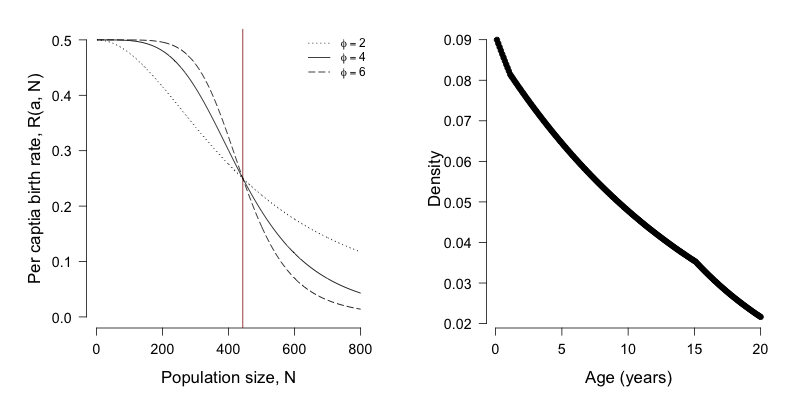
\includegraphics[width = \textwidth]{FigureS3_BH_and_agestructure.png}
  \caption*{\textbf{Fig S3.} (left) The per-capita birth rate decreases with increasing population size.  Increasing the abruptness parameter, $\phi$, results in stronger density dependence around, $K$ (red line). (right) The stable age distribution in the absence of infections appears visually similar to field estimates \cite{jolles_population_2007, caron_ecological_2003}. }
\end{figure}



\begin{table} %hb
\caption*{\textbf{Table S3.} Notation used for model variables and parameters.}
\newcommand{\head}[1]{\textnormal{\textbf{#1}}}
\small
\begin{tabular}{ll} %{12cm}
\hline
\head{Symbol} & \head{Definition}\\
\hline
\textbf{Variables} &   \\
$S(t, a)$ & buffalo susceptible to both infections of age a at time t  \\
$I_T(t, a)$ & buffalo infected with BTB only of age a at time t  \\
$I_B(t, a)$ & buffalo infected with brucellosis only and infectious of age a at time t \\
$I_C(t, a)$ & buffalo co-infected with both pathogens of age a at time t  \\
$R_B(t, a)$ & buffalo persistently infected with brucellosis but no longer infectious of age a at time t  \\
$R_C(t, a)$ & buffalo persistently infected with brucellosis and co-infected with BTB of age a at time t \\
& \\
\textbf{Parameters} &   \\
$b(a)$ & age-specific maximum birth rate at low population size\\
$K $& scaling parameter defining the characteristic population size \\
$\phi $& abruptness parameter controlling the strength of density dependence around K \\ 
$\mu_S(a) $& age-specific mortality rate for susceptible buffalo \\ 
$\mu_T(a) $& age-specific mortality rate for buffalo with BTB only \\ 
$\mu_B(a) $& age-specific mortality rate for buffalo with brucellosis \\ 
$\mu_C$ &age-specific mortality rate for buffalo co-infected with both pathogens \\ 
$\beta_T $ & transmission rate for BTB in susceptible buffalo \\
$\beta_B(a)$ & transmission rate for brucellosis in susceptible buffalo \\
$\beta_{T}^{'}$  & transmission rate for BTB in buffalo with brucellosis \\
$\beta_{B}^{'}$  & transmission rate for brucellosis in buffalo with bTB \\
$\gamma$& recovery rate for brucellosis \\
$\epsilon$& recrudescence rate for brucellosis \\
\hline 
\end{tabular}
\end{table}


\begin{table} %[H]
%\label {Table S4}
\caption*{ \textbf{Table S4.} Parameter values, dimensions, and references.}
\newcommand{\head}[1]{\textnormal{\textbf{#1}}}
\small
\begin{tabular}{llcc} %{12cm}
\hline
\head{Parameter} & \head{Value} & \head{Dimensions} & \head{Reference}\\*
\hline
$b(a)$ & 0.5 if $a \geq 5$, 0 otherwise & $yr^{-1}$ & - \\*
$K $& 433 & indiv & \cite{cross_assessing_2006} \\*
$\phi $& 4 & dimensionless & \cite{cross_assessing_2006} \\* 
$\mu_S(a) $& 0.06 if $2 < a \leq 16$, 0.1 otherwise & $yr^{-1}$ & \cite{cross_assessing_2006, jolles_hidden_2005} \\* 
$\mu_T(a) $& $2.82 \mu_S(a)$ & $yr^{-1}$ & Table S1 \\* 
$\mu_B(a) $& $3.02 \mu_S(a)$ & $yr^{-1}$ & Table S1 \\ 
$\mu_C$ & $8.58 \mu_S(a)$ & $yr^{-1}$ & Table S1 \\ 
$\beta_T $ & $1.331 * 10 ^{-4}$ & $indiv^{-1}day^{-1}$ & fit \\
$\beta_B(a)$ & $0.576$ if $a\geq 5$, $0.576 exp(0.885)$ otherwise & $day^{-1}$ & fit, Table S2 \\
$\beta_{T}^{'}$  & $\beta_T$ & $indiv^{-1}day^{-1}$ & Table S2 \\
$\beta_{B}^{'}$  & $2.09 \beta_{B}(a)$ & $day^{-1}$ & Table S2 \\
$\gamma$& 0.5 & $day^{-1}$ & \cite{rhyan_pathogenesis_2009} \\
$\epsilon$& 0.3 & $day^{-1}$ & \cite{hobbs_state-space_2015, treanor_vaccination_2010, ebinger_simulating_2011} \\
\hline 
\end{tabular}
\end{table} 

\pagebreak

\noindent
These assumptions give the following system of partial differential equations, \\
\begin{align*}
\Big \{ \frac{\partial}{\partial t} + \frac{\partial}{\partial a} \Big \} S_{}(t, a) &= r(a, N(t)) - (\lambda_{T}(t) + \lambda_{B}(t, a) + \mu_{S}(a)) S(t, a) \\*         
\Big \{ \frac{\partial}{\partial t} + \frac{\partial}{\partial a} \Big \} I_{T}(t, a)&= \lambda_{T}(t) S(t, a) -  (\lambda'_{B}(t, a) - \mu_{T}(a)) I_{T}(t, a) \\*
\Big \{ \frac{\partial}{\partial t} + \frac{\partial}{\partial a} \Big \}  I_{B}(t, a)&=  \lambda_{B}(t, a) S(t, a) - (\lambda'_{T}(t) + \gamma + \mu_{B}(a)) I_{B}(t, a) + \epsilon R_{B}(t, a) \\*
\Big \{ \frac{\partial }{\partial t} + \frac{\partial}{\partial a} \Big \}  I_{C}(t, a)&= \lambda'_{T}(t) I_{B}(t,a) + \lambda'_{B}(t, a) I_{T}(t, a) + \epsilon R_{C}(t, a) - (\gamma + \mu_{C}(a)) I_{C}(t, a) \\*
\Big \{ \frac{\partial}{\partial t} + \frac{\partial}{\partial a} \Big \}  R_{B}(t, a)&=  \gamma I_{B}(t, a) - (\epsilon + \mu_{B}(a)) R_{B}(t, a) \\*            
\Big \{ \frac{\partial}{\partial t} + \frac{\partial}{\partial a} \Big \} R_{C}(t, a)&=  \lambda'_{T} R_{B}(t, a) + \gamma I_{C}(t, a) - (\epsilon + \mu_{C}(a)) R_{C}(t, a) \\* 
\end{align*}

\noindent
with force of infection, \\*
\begin{align*}
\lambda_{T}(t) &= \beta_T \int_{0}^{\infty} (I_t(t,\alpha) + I_{C}(t,\alpha) + R_{C}(t, \alpha)) d\alpha\\*
\lambda'_{T}(t) &= \beta'_T \int_{0}^{\infty} (I_t(t,\alpha) + I_{C}(t,\alpha) + R_{C}(t, \alpha)) d\alpha\\*
\lambda_{B}(t, a) &= \beta_{B}(a) \int_{0}^{\infty} (I_{B}(t,\alpha) + I_{C}(t,\alpha)) d\alpha\\*
\lambda'_{B}(t, a) &= \beta'_{B}(a) \int_{0}^{\infty} (I_{B}(t,\alpha) + I_{C}(t,\alpha)) d\alpha\\*
\end{align*}


We used this model to investigate the consequences of co-infection for Ro and endemic infection prevalence. 
We evaluated the consequences of co-infection by comparing infection levels in scenarios where both diseases were present to scenarios with a single infection.
We calculated endemic infection levels numerically using the method-of-lines with the ode.1D function in the deSolve package in R \cite{desolve_package}.
We calculated Ro numerically using the next generation method \cite{van_den_driessche_reproduction_2002}, reviewed in \cite{heffernan_perspectives_2005}.

\section {Model sensitivity and uncertainty analysis }
We used Monte Carlo simulation to incorporate uncertainty in the individual-level consequences of co-infection quantified in our data analyses. %into predictions of $R_o$ and endemic prevalence. 
Parameter estimates from Cox proportional hazards models are normally distributed with means and standard errors provided in tables S1 and S2. We drew 1000 random parameter values following the sampling distributions in table S5.
For each value, we quantified of Ro and endemic prevalence for both pathogens in populations with and without co-infection.  
Parameter values were drawn independently (Fig S4).
Because of this, some parameters with high brucellosis mortality and low facilitation with co-infection resulted in low values of brucellosis prevalence in scenarios with and without co-infection (Fig. 3).
This parameter space occurred 4\% of the time, resulting in a heavy density around no change in brucellosis prevalence with co-infection. 
BTB prevalence remained above 1\% for all parameters.

\begin{table}[H]
\caption*{ \textbf{Table S5.} Parameter values and distributions for the individual-level consequences of co-infection.}
\newcommand{\head}[1]{\textnormal{\textbf{#1}}}
\small
\begin{tabular}{llcc} %{12cm}
\hline
\head{Parameter} & \head{Calculation} & \head{Sampling distribution} \\*
\hline
Mortality in BTB$+$ buffalo ($\mu_T$) & $\mu_T (a) = \mu_S(a) * exp(\rho_1)$ & $\rho_1 \sim \mathcal{N} (\mu = 1.04, \sigma = 0.35)$  \\*
Mortality in brucellosis$+$ buffalo ($\mu_B$)& $\mu_B (a) = \mu_S(a) * exp(\rho_2)$ & $\rho_2 \sim \mathcal{N} (\mu = 1.11, \sigma = 0.35)$ \\*
Mortality in co-infected buffalo ($\mu_C$) & $\mu_C (a) = \mu_S(a) * exp(\rho_1 + \rho_2)$ & - \\* 
Increase in brucellosis transmission with BTB & $\beta'_B = exp(\rho_3) * \beta_B$ & $\rho_3 \sim  \mathcal{N} (\mu = 1.46, \sigma = 0.41)$\\* 
\hline 
\end{tabular}
\end{table} 

\begin{figure}[H]
  \centering
  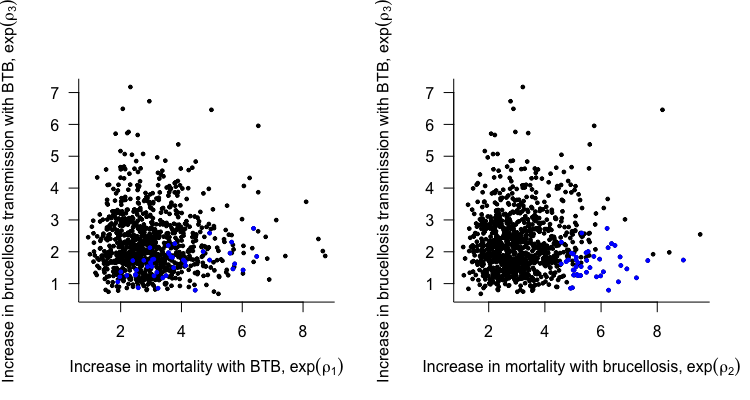
\includegraphics[width = 0.9 \textwidth]{FigureS4_MCMCparameters.png}
  \caption*{\textbf{Fig S4.} Parameter values in Table S5 were drawn independently. Blue values reflect parameters resulting in a brucellosis prevalence of $0.1\%$ or less for scenarios with and without co-infection.}
\end{figure}

We evaluated the sensitivity of our model to changes in the functional form of density dependence (Fig S5) and in parameter values (Fig S6, Fig S7). 
We used Latin Hypercube Sampling and partial rank correlation coefficients (PRCC) to quantify the strength of linear associations between model output and each parameter \cite{marino_methodology_2008}. Dots and error bars represent the partial rank correlation coefficients and $95\%$ confidence intervals based on 100 samples. Parameter ranges were drawn from a uniform distribution with ranges from 2 times greater than or less than the base values presented in Table S4.


\begin{figure}[H]
  \centering
  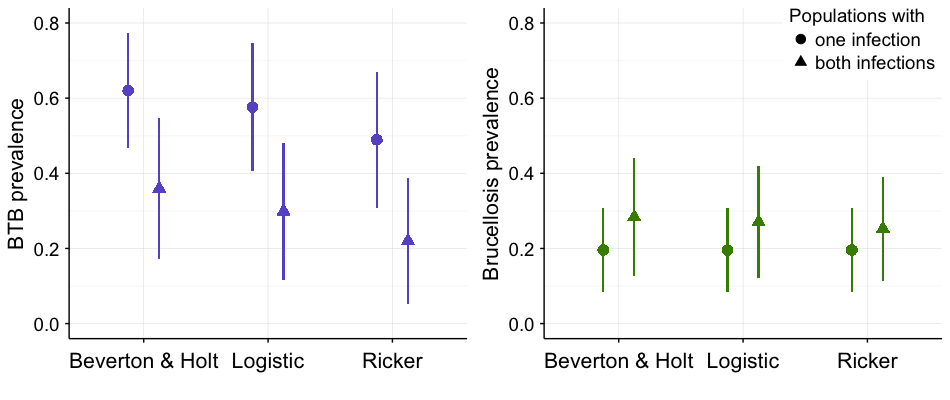
\includegraphics[width = \textwidth]{FigureS5_densitydependence.png}
  \caption*{\textbf{Fig S5.} Model results using alternative representations of density dependence, including logistic and Ricker representations. (a) Brucellosis prevalence in buffalo populations with and without co-infection. (b) BTB prevalence in buffalo populations with and without co-infection.  All three models result in similar qualitative patterns of infection and co-infection. Under the logistic and Ricker forms of density dependence, the per capita birth rate has the form, $R(a,N) = b(a) (1- \frac{N}{K_L} )$ and $R(a,N) = b(a)$exp$(\frac{-N}{K_R})$, respectively (15).  We set the parameter, K, such that all models produced the same population size in the absence of infection (609 individuals; $K_L = 1520.4$ for logistic; $K_R = 419.8 $ for Ricker).}
\end{figure}

\begin{figure}[H]
  \centering
  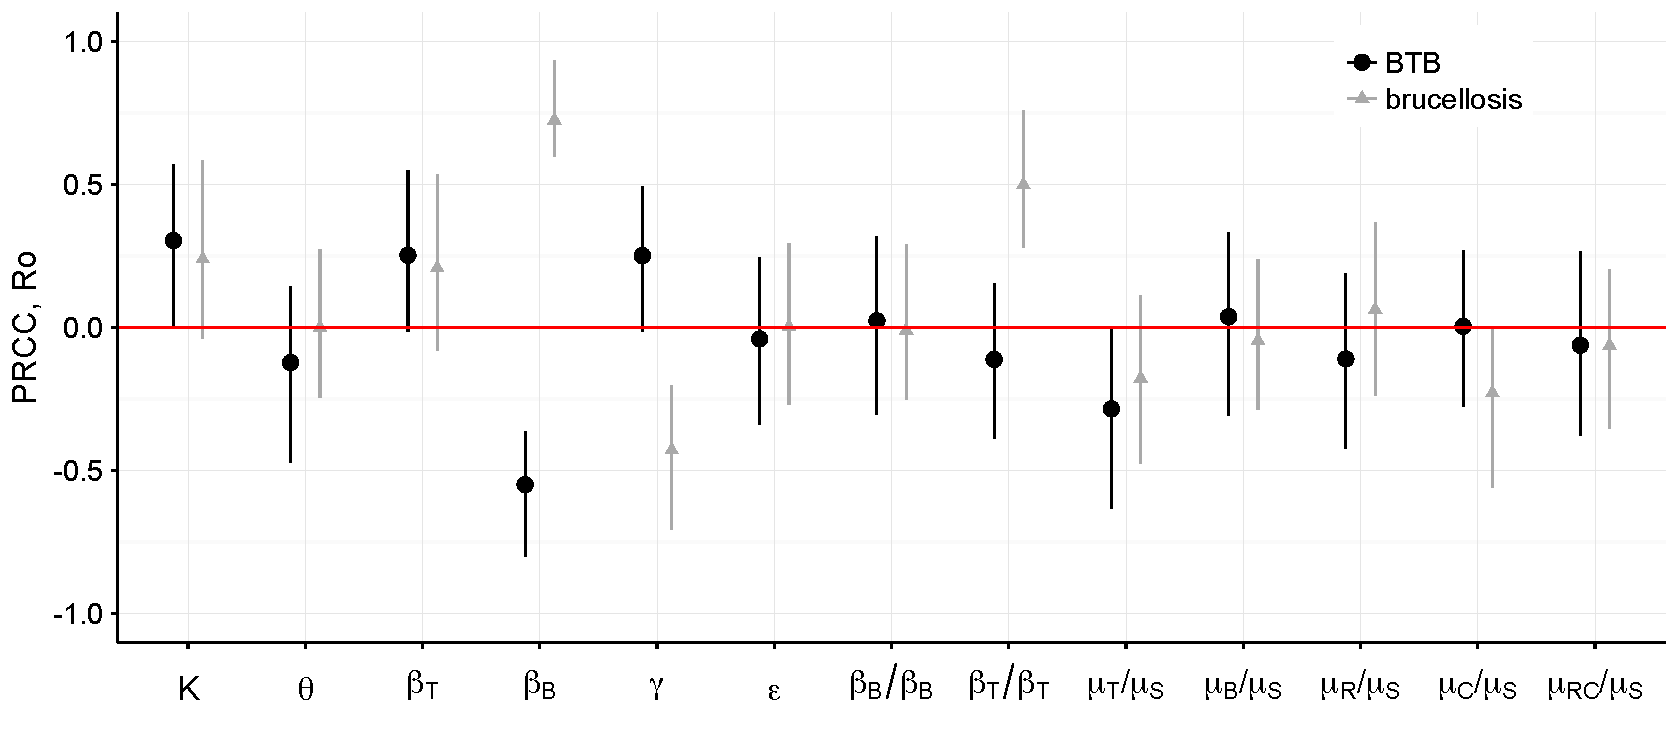
\includegraphics[width = \textwidth]{FigureS6_LHSRo_lowres.pdf}
  \caption*{\textbf{Fig S6.} Partial rank correlation coefficients and 95\% confidence intervals for $R_o$.  Colors represent the effect of a given parameter on the $R_o$ for BTB (black) or brucellosis (gray). Confidence intervals account for the 13 multiple comparisons considered here using a Bonferroni correction.}
\end{figure}

\begin{figure}[H]
  \centering
  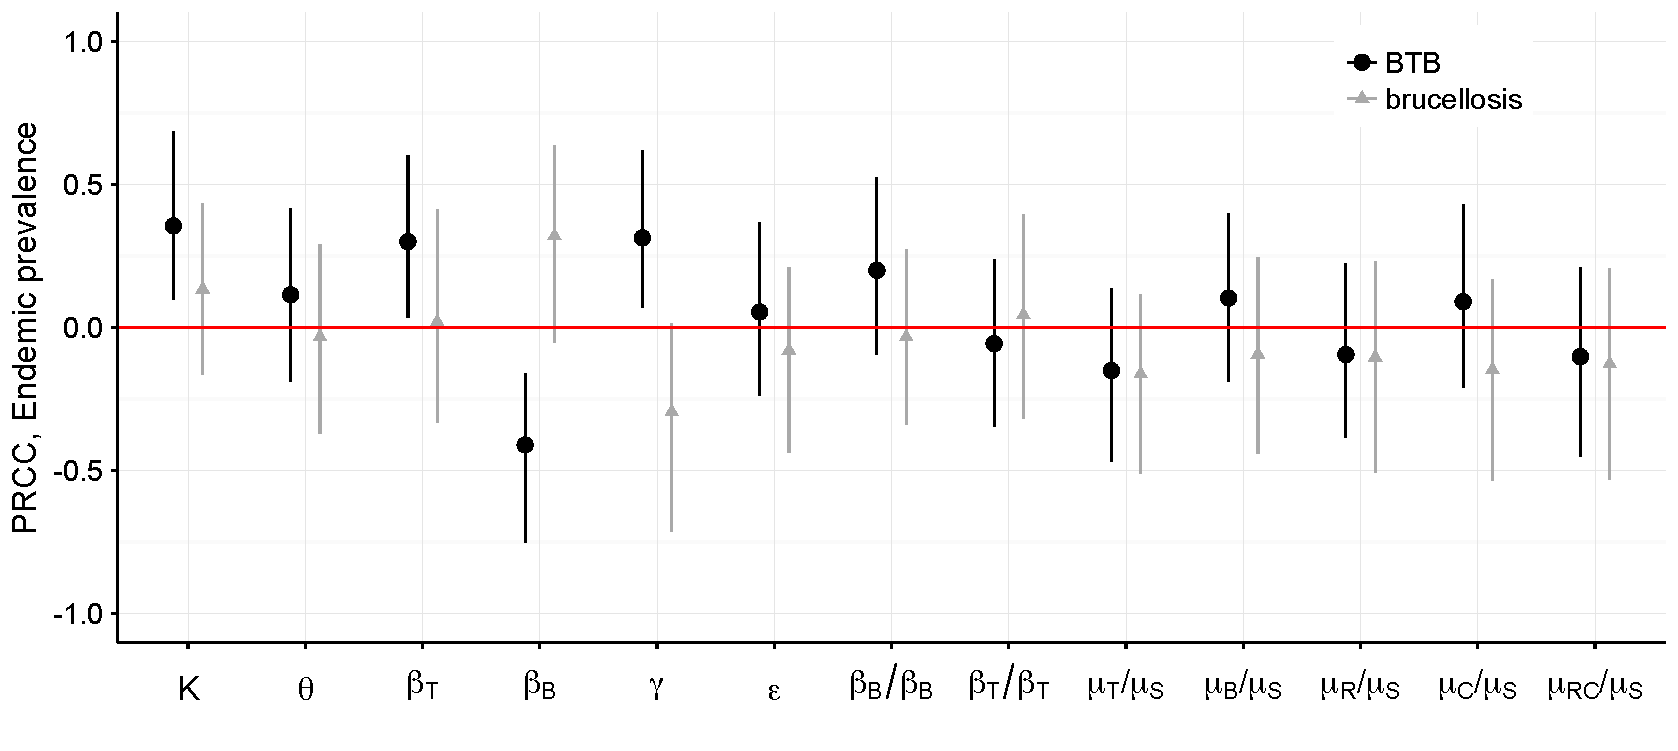
\includegraphics[width = \textwidth]{FigureS7_LHSPrev_lowres.pdf}
  \caption*{\textbf{Fig S7.} Partial rank correlation coefficients and 95\% confidence intervals for endemic prevalence.  Colors represent the effect of a given parameter on the prevalence of BTB (black) or brucellosis (gray). Confidence intervals account for the 13 multiple comparisons considered here using a Bonferroni correction.}
\end{figure}

\pagebreak

\bibliographystyle{pnas-new}
\bibliography{coinfection}




\end{document}